%!TEX root = /Users/manunavjeevan/Documents/GitHub/mnavjeev.github.io/files/Moment Inequality Methods/Annotated Literature Review/inequalityLitReview.tex

\newpage
\section{Action-Graph Games \textit{\small Albert Xin Jiang, Kevin Leyton-Brown, Navin A.R Bhat (GEB, 2011)}}
\citet{AGG-2011} appeared in \emph{Games and Economic Behavior} in 2011. It can be found online \href{https://www.sciencedirect.com/science/article/abs/pii/S0899825610001752}{here}.

\subsection{Introduction}

Simultaneous action games have received considerable study, which is reasonable as these games are fundamental. Most of the game theory literature presumes that simultaneous action games will be represented in normal form. This is problematic because, in many domains of interest, the number of players and/or the number of actions per player is large. In normal form representation, the game's payoff function is stored as a matrix with one entry for each player's payoff under each combination of all players' actions. As a result, the size of the representation grows exponentially with the number of players. 

Fortunately, most games of practical interest have highly-structured payoff functions, and thus, it is possible to represent them compactly. Intuitively, this helps to explain why people are able to reason about these games in the first place: understand the payoffs in terms of simple relationships rather than in terms of large lookup tables. One thread of recent work has explored game representations that are able to succinctly describe games of interest. For example, the extensive form allows games with temporal structure to be encoded in exponentially less space than the normal form. In what follows, however, concentrate on game representations that are compact even for simultaneous-move games of perfect information. 

Perhaps the most influential class of compact game representations is that which exploits strict independences between players' utility functions. Class includes graphical games, multi-agent influence diagrams, and game nets. Focus on the first of these. 

Consider a graph in which nodes correspond to agents and an edge from one node to another represents the proposition that the first agent is able to affect the second agents payoff's. If every node in the graph has a small in-degree, the graphical game has a compact representation (exponentially smaller than it's induced normal form). Of course, there are many ways of representing games compactly. What makes graphical games important is the fact that computational questions about these games can be answered by algorithms whose running time depends on the size of the representation rather than the size of the induced normal form. To state one fundamental property, it is possible to compute an agent's expected utility under an arbitrary mixed strategy profile in time polynomial in the size of the graphical game representation. 

This property implies that a variety of algorithms for computing game-theoretic quantities of interest, such as sample Nash and correlated equilibrium, can be made exponentially faster for graphical games without introducing any change in the algorithm's behavior or output. Property implies that a variety of algorithms for computing game-theoretic quantities of interest, such as sample Nash and correlated equilibrium can be made exponentially faster for graphical games.

A drawback of the graphical games representation is that it only helps when there exist agents who $\emph{never}$ affect some other agent' utilities. Unfortunately, many games of interest lack any structure of this kind. For example, nontrivial symmetric games are cliques when represented as graphical games. Another useful form of structure not generally captured by graphical games is dubbed \emph{anonymity}; it holds when agents utility only depends on the number of agents who took each action, rather than these agent's utilities. Recently \citet{PR-2008}, \citet{KV-200}, \citet{DP-2008}, \citet{BFH-2011}, and describe efficient computation under symmetry and anonymity.

\subsection{Action Graph Games}

Section has three parts, each of which defines a different AGG variant.

\subsubsection{Basic Action Graph Games}

Begin with an intuitive description of basic action-graph games. Consider a directed graph with nodes $\calA$ and edges $E$, and a set of agents $N = \{1, \dots, n\}$. Identical tokens are given to each agent $i \in N$. To play the game, each agent $i$ simultaneously places her token on a node $a_i \in A_i \subseteq\calA$.

Each agents utility is calculated according to an arbitrary function of the node she chose and the \emph{numbers} of tokens placed on the nodes that neighbor that chosen node in the graph.

Now argue that any simultaneous move game can be represented in this way, and that action-graph games are often much more compact than games represented in this way. To do so, need to formally define basic action-graph games. Let $N = \{1, \dots, n\}$ be the set of agents. Central to the model is the \emph{action graph}.
\begin{definition}[Action Graph]
	\label{def:AGG-2.1}
	An \underline{action graph} $G = (\calA, E)$ is a directed graph where 
	\begin{enumerate}
		\item $\calA$ is the set of nodes. Call each node $\alpha \in \calA$ an \emph{action} and the set $\calA$ the \emph{set of distinct actions}. For each agent $i \in N$, let $A_i$ be the set of actions available to $i$, with $\calA = \bigcup_{i\in N} A_i$. Denote by $a_i \in A_i$ one of agent $i$'s actions. An \emph{action profile}(or \emph{pure strategy profile}) is a tuple \(a = (a_1, \dots, a_n)\). Denote $A$ by the set of action profiles. Then $A = \prod_{i\in N} A_i$ where $\prod$ is the Cartesian product.
		\item $E$ is a set of directed edges, where self-edges are allowed. We say $\alpha'$ is a \emph{neighbor} of $\alpha$ if there is an edge from $\alpha'$ to $\alpha$, i.e $(\alpha', \alpha)\in E$. let the \emph{neighborhood} of $\alpha$, denoted $\nu(\alpha)$ be the set of neighbors of $\alpha$, i.e $\nu(\alpha) = \{\alpha'\in\calA|(\alpha',\alpha)\in E\}$
	\end{enumerate}
\end{definition}

Given an action graph and set of agents, can further define a \emph{configuration}, which is a feasible arrangement of agents across nodes in an action graph. 
\begin{definition}[Configuration]
	\label{def:AGG-2.2}
	Given an action graph $(\calA, E)$, and a set of action profiles $A$, a \underline{configuration} is a tuple of $|\calA|$ non-negative integers $(c(\alpha))_{\alpha \in \calA}$, where $c(\alpha)$ is interpreted as the number of agents who chose action $\alpha \in \calA$ and where there exists some $a \in A$ that would give rise to $c$. Denote the set of all configurations with $C$. Let $\calC:A\to C$ be the function that maps from an action profile $a$ to the corresponding configuration $c$. Formally, if $c = \calC(a)$ then $c(\alpha) = |\{i\in N: a_i = \alpha\}|$, for all $\alpha \in \calA$.
\end{definition}

 \begin{definition}[Configuration Over a Neighborhood]
 	\label{def:AGG-2.3}
 	Given a configuration $c\in C$ and a node $\alpha \in \calA$, let the \underline{configuration over the neighborhood} of $\alpha$, denoted by $c^{(\alpha)}$ be the restriction of $c$ to $v(\alpha)$, i.e $c^{(\alpha)} = (c(\alpha'))_{\alpha'\in \nu(\alpha)}$. Similarly, let $C^\Palpha$ denote the set of configurations over $\nu(\alpha)$ such that at least one platers plays $\alpha$. Let $\calC^\Palpha$
 \end{definition}

\begin{definition}[Basic Action-Graph Game]
	\label{def:AGG-2.4}
	A \underline{basic action-graph game} (AGG-$\emptyset$) is a tuple $(N, A, G, u)$ where 
	\begin{enumerate}
		\item \(N\) is the set of agents 
		\item \(A = \prod_{i\in N}A_i\) is the set of action profiles 
		\item \(G = (\calA, E)\) is an action graph where \(\calA = \bigcup_{i\in N}A_i\) is the set of distinct actions 
		\item \(u\) is a tuple \((u^\alpha)_{\alpha \in \calA}\) where each \(u^\alpha : C^\Palpha \to \SR\) is the \emph{utility function} for action \(\alpha\). Semantically, \(u^\alpha(c^\Palpha)\) is the utility of an agent who chose \(\alpha\) when the configuration over \(\nu(\alpha)\) is \(c^\Palpha\).
	\end{enumerate}
\end{definition}
For notational convenience, define \(u(\alpha, c^\Palpha)\equiv u^\alpha(c^\Palpha)\) and \(u_i(a) \equiv u(a_i, \calC^{(a_i)}(a))\)
\begin{example}[Ice Cream Vendors]
	Consider a setting in which $n$ vendors sell ice cream or strawberries and must choose one of four locations along a beach. There are three kinds of vendors: $n_I$ ice cream vendors, $n_S$ strawberry vendors and $n_W$ vendors who sell both, but only on the west side. Ice cream (strawberry) vendors are negatively affected by the presence of other ice cream (strawberry) vendors in the same or neighboring locations, and are simultaneously positively affected by the presence of nearby strawberry vendors. 
	\begin{figure}[htb!]
		\centering
		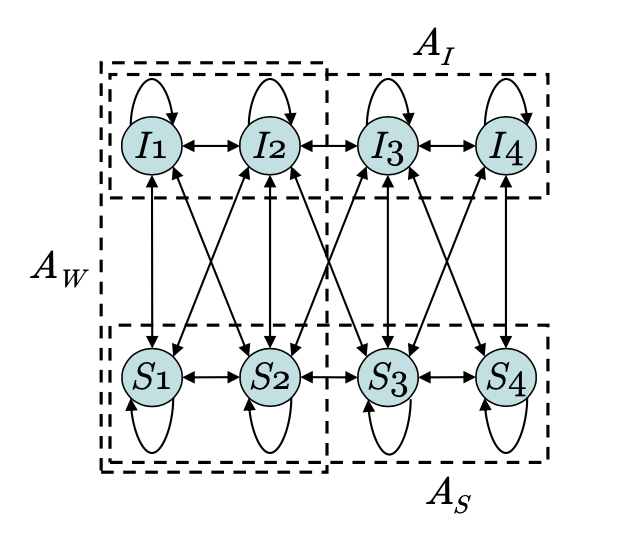
\includegraphics[width=0.4\textwidth]{figures/AGG-Fig1.png}
		\caption{AGG-\(\emptyset\) representation of the Ice Cream Vendor Game}
		\label{fig:AGG-Fig1}
	\end{figure}

	The AGG-\(\emptyset\) representation is illustrated in Figure~\ref{fig:AGG-Fig1}. It is important for computation that this representation does not depend on the number of players $n$. Nodes represent actions and directed edges represent membership in a node's neighborhood. Dotted boxes represent the action sets for each group of players; for example, the ice cream vendors have action set $A_I$.
\end{example}

\subsubsection{Size of an AGG-\texorpdfstring{\(\emptyset\)}{} Representation}

Intuitively, AGG-\(\emptyset\)s capture two types of structure in games:
\begin{enumerate}
	\item Shared actions capture the games \emph{anonymity} structure: agent $i$'s utility depends only on her action $a_i$ and the configuration. Thus, agent $i$ cares about the \emph{number} of platers that play each action, but not the identities of those players. 
	\item The (lack of) edges between nodes in the action graph expresses context-specific independencies of utilities of the game: for all $i \in N$, if $i$ chose action $\alpha \in \calA$, then $i$'s utility depends only on the configuration in $\nu(\alpha)$.
\end{enumerate}

Claimed informally that this provides a way or representing games compactly. What exactly is the size of the AGG-\(\emptyset\) representation and how does it grow with $n$. This section gives a bound and shows that it is asymptotically never worse than the size of the equivalent normal form. 

From Definition~\ref{def:AGG-2.4} observe that to completely specify an AGG-\(\emptyset\) need to specify (1) the set of agents, (2) each agent's set of actions, (3) the action graph, and (4) the utility functions. The first three can easily be compactly represented. 
\begin{enumerate}
	\item The set of agents $N = \{1, \dots, n\}$ can be specified by the integer $n$
	\item The set of actions $\calA$ can be specified by the integer $|\calA|$. Each agent's action set $A_i \subseteq \calA$ can be specified in $O(|\calA|)$ space. 
	\item The action graph $G = (\calA, E)$ can be straightforwardly represented as neighbor lists. For each node $\alpha \in \calA$, specify its list of neighbors $\nu(\alpha) \subseteq \calA$. The space required is $\sum_{\alpha \in \calA} |\nu(\alpha)|$ which is bounded by $|\calA|\calI$ where $\calI = \max_\alpha|\nu(\alpha)|$, i.e the maximum in degree of $G$.
\end{enumerate}
Observe that while the first three components of an AGG-\(\emptyset\) can always be represented in space polynomial in $n$, and $|A_i|$, the size of the utility functions is worst-case exponential. So, the size of the utility functions determines whether an AGG-\(\emptyset\) can be tractably represented. For the rest of article, refer to the number of payoff values stored as the representation size of the AGG-\(\emptyset\). The following proposition gives an upper bound on the number of payoff values stored. 

\begin{prop}
	\label{prop:AGG-2.6}
	Given an AGG-$\emptyset$ the number of payoff values stored by it's utility function is at most \(|\calA|\frac{(n-1+\calI)!}{(n-1)!\calI!}\). If $\calI$ is bounded by a constant as $n$ grows, the number of payoff values is $O(|\calA|n^\calI)$, i.e is polynomial w.r.t $n$.
\end{prop}
\begin{proof}
	For each utility function $u^\alpha:C^\Palpha\to\SR$, need to specify a utility value for each distinct configuration $c^\Palpha \in C^\Palpha$. The set of configurations $C^\Palpha$ can be derived from the action graph and can be sorted in lexicographical order. So, we can just specify a list of $|C^\Palpha|$ utility values that correspond to the (ordered) set of configurations. In general, there is no closed from expression for $|C^\Palpha|$, the number of distinct configurations over $\nu(\alpha)$. Instead, consider the operation of extending all agents' actions sets via $\forall i: A_i \mapsto \calA$. 

	The number of configurations over $\nu(\alpha)$ under the new action sets is an upper bound on $|C^\Palpha|$. This is the number of (ordered) combinatorial compositions of $n-1$ into $|\nu(\alpha)|$+1 nonnegative integers, which is \(\binom{n-1 + |\nu(\alpha)|}{|\nu(\alpha)|} \leq \binom{n-1 + \calI}{\calI}\)
\end{proof}

For each AGG-\(\emptyset\) there exists a unique \emph{induced normal form} representation with the same set of players and $|A_i|$ actions for each $i$.


